%!TEX program = xelatex
\documentclass[a4paper,UTF8]{ctexart}

\usepackage{fontspec}
\usepackage{amsmath}
\usepackage{float}
\usepackage{graphicx}
\usepackage{amssymb}
\usepackage{epstopdf}
\usepackage{mathrsfs}
\usepackage{stmaryrd}
\usepackage{color}
\usepackage{listings}
\usepackage{ulem}
\usepackage{lmodern}
\usepackage[T1]{fontenc}
\usepackage[margin=2cm]{geometry}
\usepackage{titlesec}
\usepackage{tikz}
\usepackage{svg}
\usepackage{hyperref}
\usepackage[noblocks]{authblk}

\setlength{\parskip}{5pt}

\usepackage{MyTitle}
\titleformat{\section}[hang]{\bfseries\fontsize{16pt}{0pt}\selectfont}{\thesection}{.5em}{}{}


% 对于使用 Tex Pad 打开本 TeX 文档的用户,请使用这行代码
\usepackage[cache=false,outputdir=.texpadtmp]{minted}
% 其它用户使用这行
%\usepackage{minted}
%

%To do: 修改标题和作者及联系方式
\title{HITCON2015 Quals, Forensic250, puzzleng}

\author{胡尧}
\affil{哈尔滨工业大学,计算机科学与技术学院,huyao@hit.edu.cn}

\date{}

\begin{document}
\maketitle


%------------------------------------------------------------------------------------------------------------------------------
%------------------------------------------------------------------------------------------------------------------------------
%To do: 正文开始
%------------------------------------------------------------------------------------------------------------------------------
%------------------------------------------------------------------------------------------------------------------------------

\section{题目描述}

\begin{quizdesc}[label=Forensic 250 puzzleng]
Next Generation of Puzzle!

puzzleng-edb16f6134bafb9e8b856b441480c117.tgz
\end{quizdesc}

\section{题目分析}

  下载本题,我们拿到一个加密程序和一个加密后的数据文件,逆向加密程序,我们可以得到加密算法:

%\linespread{1}
\begin{minted}{python}
pw = sha1(password)
data = bytearray(open(infile))
piecelen = (len(data)+19) // 20

for i in range(20):
    idx = i*piecelen
    data[idx:idx+piecelen] = [c^pw[i] for c in data[idx:idx+piecelen]]

\end{minted}

  加密算法首先根据一个Password生成一个20字节长度的hash(sha1),然后用这个hash作为密钥加密明文。具体来说,算法将明文按数据流分割为20片(最后一片可能比前面的短),然后用hash的每个字节分别抑或每一片中的明文数据(同一片中的数据使用同样的字节抑或),最后得到加密后的数据。

  经过简单分析,发现明文数据实际上为一张png二值(位深为1)图片,分辨率为912x912,每一片包含39个字节。

\section{解题思路}

  解这道题,实际就是算出这个hash字符串。我们从png文件格式出发,对于包含有IHDR,IEND等英文字符的数据块,我们很容易就能计算出密钥字节,但是图片中绝大部分是IDAT数据块(像素数据),而这些数据是压缩过的,并不难根据上下文确定密钥字节,于是我们需要了解一下png图片压缩算法。

\subsection{IDAT压缩算法}

  \begin{figure}[H]
    \centering
    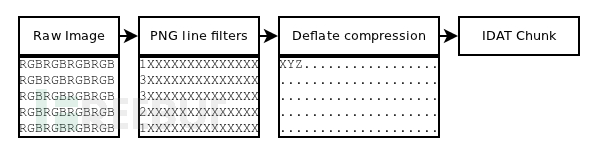
\includegraphics[width=.9\textwidth]{compress.png}
    \caption{图像数据压缩过程}\label{compress}
  \end{figure}

  如图\ref{compress},未压缩的图像数据首先会被png线性过滤器过滤一遍,然后将过滤后的数据使用Deflate算法压缩之后就得到了IDAT数据块中的内容。

  对于Deflate算法我们可以使用zlib解压。

  对于线性过滤器,通过分析png IHDR数据块,我们发现题目这种图片使用的是type 0的过滤类型,这种类型并不修改原始数据,只是在每行数据(扫描线)前面增加一个0。本图片分辨率是912x912,位深为1,所以计算出扫描线是114,经过过滤器之后,每行的数据就为115,这里可以得出一个结论,解压后数据每隔115字节数据必然会是0。

\subsection{解决办法}

  根据以上分析得到的两个信息,我们可以得出这样的解决办法:

  使用\code{zlib.decompressobj}方法从头开始一块一块递增抑或0-255所有字节暴力解压数据,当解压成功时,比较过滤器标志(每隔115字节会出现一个0),满足为0的条件时,认为解压正确(过程中可能会出现多个可能性,需要手工排除),解压下一块。这样解压得到原始图片数据,并计算出了hash。

\subsection{Flag}

  解压后图片为一个二维码,扫描后得到flag:\code{hitconqrencode -s 16 -o flag.png -l H --foreground 8F77B5 --background 8F77B4}
  

\end{document}
